\titlehead{
\vspace{-2cm}
\begin{center}
 
\includegraphics[scale=2]{Bilder/Otto_neu.eps}
\end{center}
\vspace{1cm}
}
\subject{\LARGE Masterarbeit\vspace{-5mm}}
\title{\huge Lighthouse Keeper \\ \LARGE Ein neues Verfahren zur Planung und \\ Evaluation von Beacon-Konfigurationen\\
\vspace{1mm}
\textnormal{\small von}\vspace{-1cm}}
\author{\textnormal{\large André Alexander Pieper} \\[-3.5mm] \textnormal{\large Geb. 28.03.1988 in Berlin} \\[-3.5mm] \textnormal{\large Matrikelnummer: 184960} \vspace{0.5cm}}
\date{04. Mai 2015}
\publishers{
\begin{figure}[b!]
$\begin{minipage}{12.3cm}
	\vspace{0.5cm}
	\begin{normalsize}
	\begin{tabular}[h]{ll}
	Erstprüfer: & Jun.-Prof. Dr.-Ing. Sebastian Zug \\
	& Otto-von-Guericke-Universität \\
	& Fakultät für Informatik \\
	& Institut für Verteilte Systeme \\
	& Lehrstuhl Embedded Smart Systems \\
	& Universitätsplatz 2, D-39106, Magdeburg \\ \\

	Zweitprüfer: & Prof. Dr.-Ing. Abbas Omar \\
	& Otto-von-Guericke-Universität \\
	& Fakultät für Elektro- und Informationstechnik \\
	& Institut für Informations- und Kommunikationstechnik\\
	& Lehrstuhl für Hochfrequenz- und Kommunikationstechnik \\
	& Universitätsplatz 2, D-39106, Magdeburg 
	\end{tabular}
	\end{normalsize}
\end{minipage}
\hfill
\noindent\begin{minipage}{3cm}\raggedleft\vspace{0.2cm}
 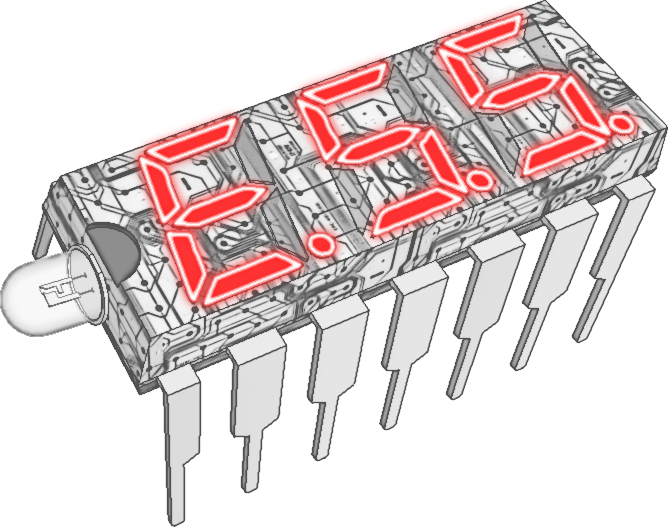
\includegraphics[scale=0.2]{Bilder/ESS.png} \\[1.3cm]
 
\includegraphics[scale=0.2]{Bilder/IIKT.png}
\end{minipage}$
\end{figure}
}

\begin{document}
\maketitle 
\newpage\thispagestyle{empty}~
\newpage
\setcounter{tocdepth}{2}
\pagenumbering{Roman}

\chapter*{Kurzdarstellung}
Satellitengestütze Navigationssysteme sind in der heutigen Zeit ein fester Bestandteil des alltäglichen Lebens. Sie ermöglichen zum Beispiel die Orientierung eines Autofahrers auf ihm unbekannten Straßen und sind mittlerweile serienmäßig in Autos, Smartphones und sogar Kameras integriert. Aber die Signale der satellitengestützten Lokalisierungssysteme wie dem "`Global Positioning System"' (GPS), "`Globalnaja nawigazionnaja sputnikowaja sistema"' (GLONASS) und "`Galileo"' verlieren sich in Gebäuden, da sie von deren Materialien absorbiert bzw. reflektiert werden. So wie die "`Outdoor"'-Lokalisierungssysteme den Straßenverkehr revolutionierten, soll ein neues "`Indoor"'-System die Fortbewegung von Menschen in Gebäuden neu erfinden: die "`Beacons"' oder zu Deutsch "`Leuchtfeuer"'. Obwohl bereits viele Unternehmen diese Technik herstellen und vermarkten, existiert im Moment noch kein zufriedenstellendes Konzept, das eine Möglichkeit bietet die nötige Infrastruktur für ein Lokalisierungssystem basierend auf Beacons effizient zu planen und zu testen. Um das Potential dieser aufstrebenden Technologie auszuschöpfen, liegt der Forschungsschwerpunkt der folgenden Ausführungen auf der Entwicklung eines dafür möglichen Verfahrens und dessen Automation mithilfe von Robotern. In Anspielung auf die Bedeutung der Beacons wird das Gesamtkonzept als "`Lighthouse Keeper"' benannt -- frei übersetzt "`Herr der Leuchtfeuer"'.